\chapter{Wstęp}

\section{Używany sprzęt oraz narzędzia}

\begin{itemize}
    \item Stanowisko - \textbf{7}
    \item Oscyloskop - \textbf{MSO3012}
    \item Generator funkcyjny - \textbf{AFG3022B}
    \item Płytka - \textbf{UC-2}
    \item Multimetr - \textbf{3}
\end{itemize}

\section{Jednostki i przedrostki}

\begin{itemize}
    \item 1 Hz (herc) - jednostka miary częstotliwości - 1Hz = $\frac{1}{1s} = 1s^{-1}$
    \item 1 V (wolt) - jednostka potencjału elektrycznego, napięcia elektrycznego i siły elektromotorycznej - 1V = $\frac{1W}{1A}$ ($\frac{wat}{amper}$)
\end{itemize}

\begin{itemize}
    \item k (kilo) = $10^3$
    \item M (mega) = $10^6$
    \item m (mili) = $10^{-3}$
    \item $\mu$ (micro) = $10^{-6}$
    \item n (nano) = $10^{-9}$
\end{itemize}

\section{Charakterystyka układów TTL}
\label{TTL:charakterystyka}

\begin{itemize}
    \item układy pracują w logice dodatniej
    \item logicznemu zeru (L – stan niski) odpowiada napięcie z przedziału:
        \begin{center}
             0 – 0.8 V (sygnały wejściowe) \\
             0 – 0.4 V (sygnały wyjściowe)
        \end{center}
    \item logicznej jedynce (H – stan wysoki) odpowiada napięcie z zakresu:
        \begin{center}
            2.0 – 5 V (sygnały wejściowe) \\
            2.7 – 5 V (sygnały wyjściowe)
        \end{center}
    \item wejście bramki niepodłączone do niczego znajduje się w stanie logicznym 1
    \item układy zasila się napięciem +5 V.
\end{itemize}

\pagebreak

\section{Bramki logiczne}

\begin{itemize}
    \item Bramka NOT:
        \begin{itemize}
            \item Symbol:
                \begin{figure}[H]
                    \centering
                    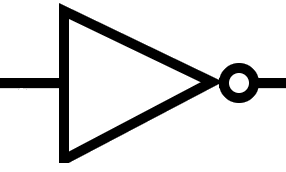
\includegraphics[scale=0.5]{img/schemes/NOT_symbol.png}
                    \caption{Symbol bramki NOT}
                    \label{fig:symbol_NOT}
                \end{figure}
            \item Wyrażenie algebraiczne:
                \begin{equation}
                    \label{eq:NOT}
                    Y = \Bar{A}
                \end{equation}
            \item Tabela prawdy:
            \begin{center}
                \label{tabela_prawdy:NOT}
                \begin{tabular}{|c|>{\columncolor[gray]{0.8}}c|}
                    \hline
                    A & Y \\
                    \hline
                    0 & 1 \\
                    \hline
                    1 & 0 \\
                    \hline
                \end{tabular}
            \end{center}
        \end{itemize}
        
    \item Bramka OR:
        \begin{itemize}
            \item Symbol:
                \begin{figure}[H]
                    \centering
                    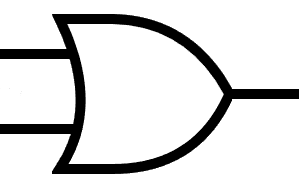
\includegraphics[scale=0.5]{img/schemes/OR_symbol.png}
                    \caption{Symbol bramki OR}
                    \label{fig:symbol_OR}
                \end{figure}
            \item Wyrażenie algebraiczne:
                \begin{equation}
                    \label{eq:OR}
                    Y = A+B
                \end{equation}
            \item Tabela prawdy:
            \begin{center}
                \label{tabela_prawdy:OR}
                \begin{tabular}{|c|c|>{\columncolor[gray]{0.8}}c|}
                    \hline
                    A & B & Y \\
                    \hline
                    0 & 0 & 0 \\
                    \hline
                    0 & 1 & 1 \\
                    \hline
                    1 & 0 & 1 \\
                    \hline
                    1 & 1 & 1 \\
                    \hline
                \end{tabular}
            \end{center}
        \end{itemize}
        
\pagebreak

    \item Bramka NOR:
        \begin{itemize}
            \item Symbol:
                \begin{figure}[H]
                    \centering
                    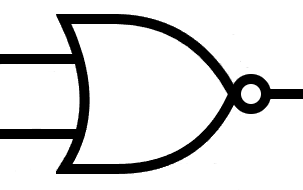
\includegraphics[scale=0.5]{img/schemes/NOR_symbol.png}
                    \caption{Symbol bramki NOR}
                    \label{fig:symbol_NOR}
                \end{figure}
            \item Wyrażenie algebraiczne:
                \begin{equation}
                    \label{eq:NOR}
                    Y = \overline{A + B}
                \end{equation}
            \item Tabela prawdy:
            \begin{center}
                \label{tabela_prawdy:NOR}
                \begin{tabular}{|c|c|>{\columncolor[gray]{0.8}}c|}
                    \hline
                    A & B & Y \\
                    \hline
                    0 & 0 & 1 \\
                    \hline
                    0 & 1 & 0 \\
                    \hline
                    1 & 0 & 0 \\
                    \hline
                    1 & 1 & 0 \\
                    \hline
                \end{tabular}
            \end{center}
        \end{itemize}
        
    \item Bramka AND:
        \begin{itemize}
            \item Symbol:
                \begin{figure}[H]
                    \centering
                    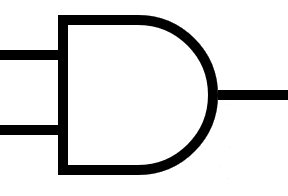
\includegraphics[scale=0.5]{img/schemes/AND_symbol.png}
                    \caption{Symbol bramki AND}
                    \label{fig:symbol_AND}
                \end{figure}
            \item Wyrażenie algebraiczne:
                \begin{equation}
                    \label{eq:AND}
                    Y = AB
                \end{equation}
            \item Tabela prawdy:
            \begin{center}
                \label{tabela_prawdy:AND}
                \begin{tabular}{|c|c|>{\columncolor[gray]{0.8}}c|}
                    \hline
                    A & B & Y \\
                    \hline
                    0 & 0 & 0 \\
                    \hline
                    0 & 1 & 0 \\
                    \hline
                    1 & 0 & 0 \\
                    \hline
                    1 & 1 & 1 \\
                    \hline
                \end{tabular}
            \end{center}
        \end{itemize}
        
\pagebreak
        
    \item Bramka NAND:
        \begin{itemize}
            \item Symbol:
                \begin{figure}[H]
                    \centering
                    \includegraphics[scale=0.5]{img/schemes/nand_symbol.png}
                    \caption{Symbol bramki NAND}
                    \label{fig:symbol_NAND}
                \end{figure}
            \item Wyrażenie algebraiczne:
                \begin{equation}
                    \label{eq:NAND}
                    Y = \overline{AB}
                \end{equation}
            \item Tabela prawdy:
            \begin{center}
                \label{tabela_prawdy:NAND}
                \begin{tabular}{|c|c|>{\columncolor[gray]{0.8}}c|}
                    \hline
                    A & B & Y \\
                    \hline
                    0 & 0 & 1 \\
                    \hline
                    0 & 1 & 1 \\
                    \hline
                    1 & 0 & 1 \\
                    \hline
                    1 & 1 & 0 \\
                    \hline
                \end{tabular}
            \end{center}
        \end{itemize}
        
    \item Bramka XOR:
        \begin{itemize}
            \item Symbol:
                \begin{figure}[H]
                    \centering
                    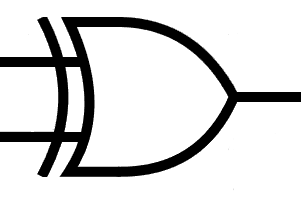
\includegraphics[scale=0.5]{img/schemes/XOR_symbol.png}
                    \caption{Symbol bramki XOR}
                    \label{fig:symbol_XOR}
                \end{figure}
            \item Wyrażenie algebraiczne:
                \begin{equation}
                    \label{eq:XOR}
                    Y = A \oplus B
                \end{equation}
            \item Tabela prawdy:
            \begin{center}
                \label{tabela_prawdy:XOR}
                \begin{tabular}{|c|c|>{\columncolor[gray]{0.8}}c|}
                    \hline
                    A & B & Y \\
                    \hline
                    0 & 0 & 0 \\
                    \hline
                    0 & 1 & 1 \\
                    \hline
                    1 & 0 & 1 \\
                    \hline
                    1 & 1 & 0 \\
                    \hline
                \end{tabular}
            \end{center}
        \end{itemize}
\end{itemize}

\pagebreak

\section{Czas propagacji}

\begin{itemize}
    \item Jest to czas upływający od chwili zmiany stanu wejścia układu logicznego lub elementu logicznego do chwili ustalenia stanu wyjść, będącej reakcją na tę zmianę wejścia.
    \item Dla przejścia ze stanu niskiego do wysokiego (oznaczany $t_{pLH}$)
    \item Dla przejścia ze stanu wysokiego do niskiego (oznaczany $t_{pHL}$)
    \item Średni czas propagacji:
        \begin{equation}
            \label{propagacja:sredni_czas} t_p = \dfrac{t_{pLH}+t_{pHL}}{2}
        \end{equation}
    \item Wyznaczanie czasu propagacji:
        \begin{figure}[H]
            \centering
            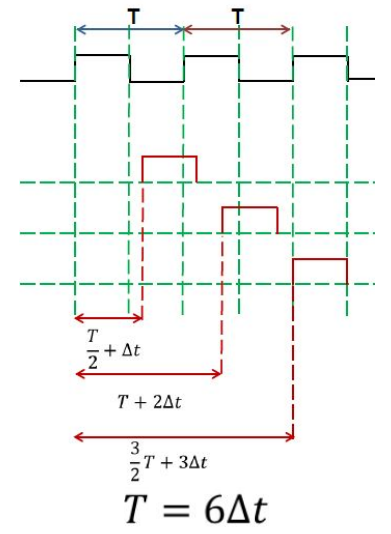
\includegraphics[scale=0.8]{img/schemes/wyznaczanie_czasu_propagacji.png}
            \label{propagacja:wyznaczanie_czasu_propagacji}
        \end{figure}
\end{itemize}

\pagebreak

\section{Przerzutnik asynchroniczny R-S}

\begin{itemize}
    \begin{figure}[H]
        \centering
        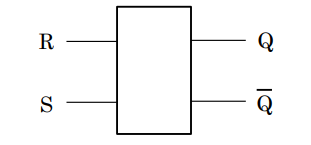
\includegraphics[scale=0.5]{img/schemes/RS_schemat.png}
        \caption{Ogólny schemat przerzutnika R-S}
        \label{przerzutnik:ogolny_schemat}
    \end{figure}
    \item Posiada:
        \begin{itemize}
            \item dwa wejścia:
                \begin{center}
                    \textbf{S (Set)} – wejście ustawiające \\
                    \textbf{R (Reset)} – wejście zerujące
                \end{center}
            \item dwa wyjścia:
                \begin{center}
                    \textbf{Q – wyjście zwykłe} (główne) \\
                    \textbf{Q – wyjście zanegowane} (komplementarne).
                \end{center}
        \end{itemize}
    Stan wyjść jest zawsze przeciwny.
    \item Przerzutnik można ustawić w stan zero (Q=0) Q przez podanie sygnału 1 na wejście R przy S=0.
    \item Ustawienie przerzutnika w stan jeden (Q=1) realizuje się przez podanie sygnału 1 na wejście S przy R utrzymywanym w stanie 0.
    \item Po przywróceniu stanu R=0 i S=0 przerzutnik wprowadzony zostaje w stan pamiętania, przechowując ustawiony stan. W ten sposób w przerzutniku zapamiętuje się elementarną porcję (1 – bit) informacji.
    \begin{figure}[H]
        \centering
        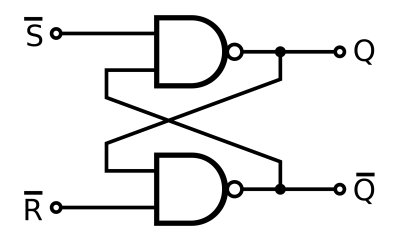
\includegraphics[scale = 0.6]{img/schemes/przerzutnik_rs_schemat.png}
        \caption{Schemat przerzutnika R-S używając bramek \textbf{NAND}}
        \label{przerzutnik:schemat}
    \end{figure}
    \item Tabela stanów:
        \begin{center}
            \label{tabela_stanow_RS}
            \begin{tabular}{|c|c|>{\columncolor[gray]{0.8}}c|}
                \hline
                \overline{S} & \overline{R} & Q \\
                \hline
                0 & 0 & stan zabroniony \\
                \hline
                0 & 1 & 1 \\
                \hline
                1 & 0 & 0 \\
                \hline
                1 & 1 & stan pamiętania \\
                \hline
            \end{tabular}
        \end{center}
\end{itemize}